
%pygmentize_options: -O startinline=True

\chapter{Abstract}
Dynamically typed programming languages have been gaining popularity 
over past years. Among them, the PHP programming language is still 
the highest ranked dynamic language in the TIOBE index \cite{tiobe}. 
The possibility to omit type information, 
% which can be
helpful during the early stages of a software project, 
can lead to more error prone code, and eventually to 
problems in later phases of the development and maintenance. 
The lack of type information also prevents compilers 
from emitting more efficient code. To overcome this problem and 
still benefit from dynamic typing, we propose to use static 
analysis methods to infer type information in PHP code where possible. 
The results of the type analysis can be then used to inform 
the programmer about possible type mismatch related errors in 
the IDE and to provide information to the compiler back-end. 
The aim of the project is to implement such analysis 
within a context of Phalanger: The PHP compiler for .NET.

%In this thesis we present our approach to 
%adapt and apply known techniques for static analysis to 
%the real world programming language PHP in the context 
%of an ongoing project Phalanger: The PHP compiler for .NET.

\chapter{Project Description}

Because of its dynamic nature, PHP code is more difficult to analyse 
than code written in a statically typed language, especially if we 
want the analysis to be reasonably fast so that it can be used 
in everyday development. There is an ongoing research of the 
static analysis methods for many different families of programming 
languages, including dynamic languages. 

The the following two sections we will discuss some of the specific 
properties of the PHP language that make any analysis of code 
written in PHP more difficult and then we will provide an overview 
of the static analysis methods.

\section{Background: PHP Programming \mbox{Language}}

The project will focus on PHP version 5.5, which is an object 
oriented dynamically typed programming language. Local or global 
variables, object fields and function or method parameters in PHP 
are dynamically typed, which means that one variable can hold 
values of completely different types during its lifetime.

\subsection{Local Variables}
Local variables in PHP do not need to be declared explicitly. 
Instead the first usage of a variable is also its declaration. 
If a variable's value is used before the variable got any 
value assigned, then the interpreter generates a notice, 
however the execution continues and value \code{null} is 
used instead. A variable can get a value assigned when it 
appears on a left hand side of an assignment or when a 
reference to that variable is created and then assigned a value. 
References are discussed in one of the following subsections.

The scope of a local variable is always its parent function not the 
code block as in other languages like C or Java. So in the following 
example, the usage of variable \code{\$y} at the end of the function 
can generate uninitialized variable notice, however, if \code{\$x} 
was equal to \code{3}, \code{\$y} will have a value although it 
was declared in a nested code block.

%pygmentize_begin php
% function foo($x) {
%   if ($x == 3) { $y = 2; }
%   echo $y; // uninitialized variable if x != 3
% }
%pygmentize_end
\begin{Verbatim}[commandchars=\\\{\}]
 \PY{k}{function} \PY{n+nf}{foo}\PY{p}{(}\PY{n+nv}{\PYZdl{}x}\PY{p}{)} \PY{p}{\PYZob{}}
   \PY{k}{if} \PY{p}{(}\PY{n+nv}{\PYZdl{}x} \PY{o}{==} \PY{l+m+mi}{3}\PY{p}{)} \PY{p}{\PYZob{}} \PY{n+nv}{\PYZdl{}y} \PY{o}{=} \PY{l+m+mi}{2}\PY{p}{;} \PY{p}{\PYZcb{}}
   \PY{k}{echo} \PY{n+nv}{\PYZdl{}y}\PY{p}{;} \PY{c+c1}{// uninitialized variable if x != 3}
 \PY{p}{\PYZcb{}}
\end{Verbatim}

\subsection{Indirect Access}
PHP allows indirect access to variables and object fields meaning 
that another variable's value can be used as a variable name in 
arbitrary expression including assignment expressions. 
Indirect access poses a challenge for any static analysis approach. 
The syntax is as follows:

%pygmentize_begin php
% $x = 'hello';
% $$x = 'world';
% echo $hello; // prints 'world'
% echo $$x;    // prints 'world' too
% echo $x;     // prints 'hello'
% $o = new Object();
% $o->{$x} = 'world';  // indirect field access
%pygmentize_end
\begin{Verbatim}[commandchars=\\\{\}]
 \PY{n+nv}{\PYZdl{}x} \PY{o}{=} \PY{l+s+s1}{\PYZsq{}hello\PYZsq{}}\PY{p}{;}
 \PY{n+nv}{\PYZdl{}\PYZdl{}x} \PY{o}{=} \PY{l+s+s1}{\PYZsq{}world\PYZsq{}}\PY{p}{;}
 \PY{k}{echo} \PY{n+nv}{\PYZdl{}hello}\PY{p}{;} \PY{c+c1}{// prints \PYZsq{}world\PYZsq{}}
 \PY{k}{echo} \PY{n+nv}{\PYZdl{}\PYZdl{}x}\PY{p}{;}    \PY{c+c1}{// prints \PYZsq{}world\PYZsq{} too}
 \PY{k}{echo} \PY{n+nv}{\PYZdl{}x}\PY{p}{;}     \PY{c+c1}{// prints \PYZsq{}hello\PYZsq{}}
 \PY{n+nv}{\PYZdl{}o} \PY{o}{=} \PY{k}{new} \PY{n+nx}{Object}\PY{p}{();}
 \PY{n+nv}{\PYZdl{}o}\PY{o}{\PYZhy{}\PYZgt{}}\PY{p}{\PYZob{}}\PY{n+nv}{\PYZdl{}x}\PY{p}{\PYZcb{}} \PY{o}{=} \PY{l+s+s1}{\PYZsq{}world\PYZsq{}}\PY{p}{;}  \PY{c+c1}{// indirect field access}
\end{Verbatim}

\subsection{References}
References in PHP are similar to pointers in C. A reference is 
created using the operator \code{\&=}, 
for example \code{\$a\&=\$b;} The left hand side is 
the reference and right hand side is where the reference 
is pointing to. After this assignment, every assignment of any 
value to \code{\$a} alternates the value of \code{\$b} and 
when when the value of \code{\$a} is to be used in an expression, 
the value of \code{\$b} is used instead.

Functions in PHP can take references, a reference may 
refer to another reference. References may refer not only to 
local variables but also to object fields and global variables. 
There are many aspects of references, that make it difficult 
to analyse PHP code if we do not want to ignore this 
language feature completely.

\section{Background: Static Analysis}
Static analysis of source code is an analysis that is performed without 
actually executing the code. This means that we do not have to have a
web server for example in order to analyse code of a web application. 
We can also guarantee some properties that would not be possible to 
guarantee if we executed the code. Namely the halting property and 
upper bounds on time and space complexity. Arbitrary code may not 
halt if executed, but static analysis of such code can still halt 
and give us some results.

There are several approaches to static analysis. Some of them are well 
established and used in many modern compilers and other tools, others 
are still in a research.

Widely used approach is a Data Flow analysis described in 
classical textbook for compiler construction \cite{aho1985compilers}. 
This approach represents a generic framework for analysis of the 
source code in a form of control flow graph with nodes representing 
blocks of code and edges representing the possible execution flow as 
depicted in the figure \ref{cfg}.

\begin{table}[h]
  \begin{tabular}{ l | p{3cm} }
  \centering
    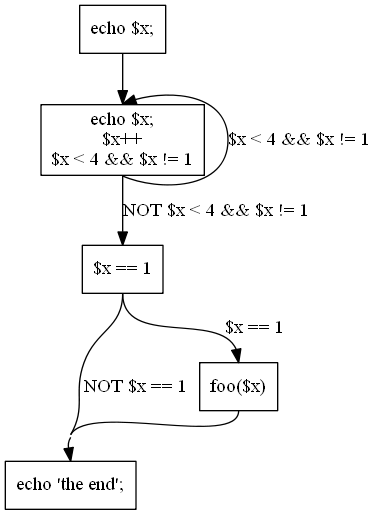
\includegraphics[scale=0.7]{cfg.png}
  &
 
 
\begin{minipage}{1in} 
\vspace{0pt}
%pygmentize_begin php
%echo $x;
%do {
%    echo $x;
%    $x++;
%} while ($x < 4 && $x != 1);
%
%if ($x == 1)
%    foo($x);
%    
%echo 'the end';
%pygmentize_end
\begin{Verbatim}[commandchars=\\\{\}]
\PY{k}{echo} \PY{n+nv}{\PYZdl{}x}\PY{p}{;}
\PY{k}{do} \PY{p}{\PYZob{}}
    \PY{k}{echo} \PY{n+nv}{\PYZdl{}x}\PY{p}{;}
    \PY{n+nv}{\PYZdl{}x}\PY{o}{++}\PY{p}{;}
\PY{p}{\PYZcb{}} \PY{k}{while} \PY{p}{(}\PY{n+nv}{\PYZdl{}x} \PY{o}{\PYZlt{}} \PY{l+m+mi}{4} \PY{o}{\PYZam{}\PYZam{}} \PY{n+nv}{\PYZdl{}x} \PY{o}{!=} \PY{l+m+mi}{1}\PY{p}{);}

\PY{k}{if} \PY{p}{(}\PY{n+nv}{\PYZdl{}x} \PY{o}{==} \PY{l+m+mi}{1}\PY{p}{)}
    \PY{n+nx}{foo}\PY{p}{(}\PY{n+nv}{\PYZdl{}x}\PY{p}{);}
    
\PY{k}{echo} \PY{l+s+s1}{\PYZsq{}the end\PYZsq{}}\PY{p}{;}
\end{Verbatim}
\vspace{5pt}
\end{minipage}

  \\
  \end{tabular}
  \caption{Control flow graph\label{cfg}}  
\end{table}

The Data Flow approach does not specify how to analyse each node 
in the control flow graph. It is up to the user to define 
the analysis and if it follows certain properties, then the 
Data Flow algorithm is guaranteed to terminate with the given 
time and space complexity that also depend on the analysis properties.

Other techniques for static analysis include 
abstract interpretation \cite{cousot1977abstract} 
and symbolic execution \cite{king1976symbolic}. 
Different methods can be combined to achieve 
the desired results. 


\section{Aims, Significance and Expected Outcomes}

The aim of the project is to provide a generic framework 
for analysing PHP source code and type analysis based on 
this framework. This should be done within the context 
of the Phalanger project \cite{benda2006phalanger} meaning 
that the framework should use the existing Phalanger parser 
and its data structures and should be designed in a way that 
it will be possible to plug it in between the Phalanger 
compiler front-end and back-end.

Type analysis results can be used to provide developers with 
a live feedback in their IDE showing possible type related 
errors. The type information can also be used to in the compiler 
back-end in order to emit more efficient code.

Aside the generic framework and library, another expected 
outcome of the project is a console application that will perform 
static type analysis on given PHP source code files and 
will print out all the discovered errors and warnings.

\chapter{Approach}

The project consists primarily of software design and development. 

\paragraph*{}
During the initial phase, methods for static analysis should be 
researched. However, the project itself is focused on providing 
a near to production ready analysis software based on existing 
research and industry practice, but not on further research 
or development of the static analysis methods.

\paragraph*{}
The features that have to be implemented can 
be split into three phases:
\begin{itemize}
    \item Extraction of control flow graph from abstract syntax tree provided by the Phalanger parser.
    \item Generic framework for Data Flow based analysis.
    \item Type analysis based on the generic framework.
\end{itemize}

\paragraph*{}
In order to provide an analysis suitable for real world usage, 
the last step will be to analyse several middle and large sized 
PHP open source projects in order to fix any bugs found, 
improve performance if needed and evaluate the project. 
Lastly the project will be compared to similar software 
projects, namely Phantm \cite{kneuss2010using} and possibly others.


\chapter{Task Plan}
The project has already been started and currently is in the 
third phase of the software development: implementation of type 
analysis based on the generic static analysis framework. 

The following table outlines all tasks. Detailed description 
is provided in the following paragraphs where needed.

\begin{center}
    \begin{tabular}{ | l | l | l | p{7cm} |}
    \hline
    ID & Name & Time Period & Deliverables\\ \hline
    
    1 & Type Analysis & Week 5 & 
        A console application that can analyse give PHP source code files.
    \\ \hline
        
    2 & Project Report Outline & Week 6 & 
        The Project Report Outline document \\ \hline
        
    3 & Project Evaluation & Weeks 7,8 &
        List of all discovered errors \\ \hline
        
    4 & Final Report & Weeks 10-13 &
        The Final Report \\ \hline        
        
    5 & Presentation & Weeks 14 &
        The Final Project Presentation \\ \hline                

    \end{tabular}
\end{center}

\section{Type Analysis}
The aim is to finish the type analysis and develop a 
console application that would provide means to run 
the analysis on specified files using different 
configurations of the analysis. I.e., 
the console application should allow to test the 
library with most of its features.

\section{Project Evaluation}
The software will be run on the source code files of 
Zend Framework, PhpUnit, Drupal and Wordpress. 
All the errors found will be categorized and recorded. 
The results will have a form of a git repository with 
all the discovered errors rectified, which will be visible 
in the commit log, and all the false positives commented in 
the source code.

\section{Final Report}
The division of this task will be determined by the outcome of 
task number 2: Project Report Outline. However, in the four 
weeks allocated for this task, I expect to write 
introduction and theoretical parts during the first week, 
implementation part in second week, 
results and conclusion in third week and 
the last week will be left for finalising the report.

